\documentclass[../../../../main.tex]{subfiles}
\begin{document}

\begin{flushright}
\footnotesize\textit{【自動文字起こし・要確認】}
\end{flushright}

[解] 原点$O$とし、点$X$の位置ベクトルを$\vec{x}$とする。

\begin{minipage}{0.5\textwidth}
$$ \begin{cases}
\vec{a}_{n+1} = (\vec{b}_n + \vec{c}_n + \vec{d}_n) / 3 \\
\vec{b}_{n+1} = (\vec{a}_n + \vec{c}_n + \vec{d}_n) / 3 \\
\vec{c}_{n+1} = (\vec{a}_n + \vec{b}_n + \vec{d}_n) / 3 \quad \cdots \text{(1)} \\
\vec{d}_{n+1} = (\vec{a}_n + \vec{b}_n + \vec{c}_n) / 3
\end{cases} $$
帰納的に
$\vec{a}_n + \vec{b}_n + \vec{c}_n + \vec{d}_n = \vec{a} + \vec{b} + \vec{c} + \vec{d} \cdots \text{(2)}$
\end{minipage}
\begin{minipage}{0.4\textwidth}
\begin{center}
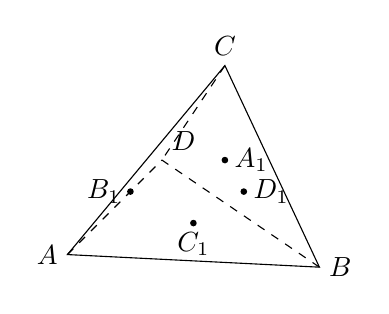
\begin{tikzpicture}[scale=0.8]
  \coordinate (A) at (0,0);
  \coordinate (B) at (4,-0.2);
  \coordinate (C) at (2.5,3);
  \coordinate (D) at (1.5,1.5);
  \draw (A) node[left] {$A$} -- (B) node[right] {$B$} -- (C) node[above] {$C$} -- cycle;
  \draw[dashed] (A) -- (D) node[above right] {$D$};
  \draw[dashed] (B) -- (D);
  \draw[dashed] (C) -- (D);
  \fill (2.5, 1.5) circle (1.5pt) node[right] {$A_1$};
  \fill (1, 1) circle (1.5pt) node[left] {$B_1$};
  \fill (2, 0.5) circle (1.5pt) node[below] {$C_1$};
  \fill (2.8, 1) circle (1.5pt) node[right] {$D_1$};
\end{tikzpicture}
\end{center}
\end{minipage}

(1) $AA_1, BB_1, CC_1, DD_1$上の点は各々 $0 \le t, s, u, v \le 1$として
$$ t \vec{a}_1 + (1-t) \vec{a} $$
$$ s \vec{b}_1 + (1-s) \vec{b} $$
$$ u \vec{c}_1 + (1-u) \vec{c} $$
$$ v \vec{d}_1 + (1-v) \vec{d} $$
で表される。$t=s=u=v=\frac{3}{4}$とすれば、いずれも
$$ \frac{1}{4} (\vec{a} + \vec{b} + \vec{c} + \vec{d}) $$
を通るから、これが$P$である (証)

(2) 帰納的に示す。つまり$A_1 A_2, A_3 \dots$が直線$AA_1$上にあることを示す。$AA_1$上の点$X$は$t \in \mathbb{R}$として
$$ \vec{x} = \frac{t}{3} (\vec{b} + \vec{c} + \vec{d}) + (1-t) \vec{a} \cdots \text{(3)} $$
と表される。$n=1$の時は明らか。$n=k$での成立を仮定する
(1), (2) から
$$ \vec{a}_{k+1} = \frac{1}{3} (\vec{a} + \vec{b} + \vec{c} + \vec{d} - \vec{a}_k) $$
カテイから、(3)で、$\vec{a}_k$に対応する$t$が存在し、これを$t_k$とおくと
$$ \vec{a}_{k+1} = \frac{1}{3} \left[ \vec{a} + \vec{b} + \vec{c} + \vec{d} - \frac{t_k}{3} (\vec{b} + \vec{c} + \vec{d}) - (1-t_k) \vec{a} \right] $$
$$ = \frac{1}{3} \left[ \left(1-\frac{t_k}{3}\right) (\vec{b} + \vec{c} + \vec{d}) + t_k \vec{a} \right] $$
だが、これは(3)で $t = 1 - \frac{t_k}{3}$ としたものにひとしく、$A_{k+1}$も$AA_1$上にある。よって$n=k+1$でも成立。
以上から示された (証)

(3) (2)から、点$A_n$に対応する$t$を$t_n$とおくと
$$ \begin{cases} t_{n+1} = 1 - \frac{t_n}{3} \\ t_1 = 1 \end{cases} $$
これをといて、等比数列の公式から、
$$ t_n = \left(-\frac{1}{3}\right)^{n-1} \left(1-\frac{3}{4}\right) + \frac{3}{4} $$
よって、$t_n \to \frac{3}{4} \ (n \to \infty)$ だから、(1)とあわせて、
$$ A_n \to P \ (n \to \infty) $$
となり
$$ \vec{A_n P} \to 0 \ (n \to \infty) $$
である (証)

\end{document}
